\begin{figure*}[h!]
\centering
\scriptsize
\definecolor{myblue}{HTML}{1A4FE0}    %
\definecolor{mypurple}{HTML}{6A3FD6}  %
\tcbset{
    promptbox/.style={
        colback=gray!5, boxrule=0.5pt, arc=1mm,
        left=1mm, right=1mm, top=0.5mm, bottom=0.5mm,
        fonttitle=\scriptsize\bfseries, valign=top,
        width=\linewidth, height=4.5cm
    },
    objbox/.style={
        promptbox, colframe=myblue, coltitle=myblue,
        colbacktitle=myblue!14
    },
    subjbox/.style={
        promptbox, colframe=mypurple, coltitle=mypurple,
        colbacktitle=mypurple!14
    },
    groupbox/.style={
        boxrule=0.5pt, arc=1mm,
        left=1mm, right=1mm, top=0.5mm, bottom=0.5mm,
        halign=center, valign=center,
        fontupper=\normalsize\bfseries,
        width=\linewidth
    }
}
\newcommand{\secskip}{\vspace{1.2pt}}

\begin{minipage}[t]{0.245\textwidth}%
\begin{tcolorbox}[objbox, title={Objective: Opinion Prompt}]%
\tiny
\textbf{Expertise}\par
You are a mathematics expert on a panel. Calibrate to this solved example: [\textit{Algebra L5 problem + ground-truth solution}].
\secskip

\textbf{Messages}\par
[messages from concordant connections]\par
[messages from discordant connections]
\secskip

\textbf{Problem}\par
[Zorn the Conqueror remainder problem] \quad A) 201 \quad B) 202
\secskip

\textbf{Instruction}\par
Give your gut answer; no reasoning or steps.
\secskip

\textbf{Format}\par
A single character: \texttt{A} or \texttt{B}.
\end{tcolorbox}%
\end{minipage}%
\hfill%
\begin{minipage}[t]{0.245\textwidth}%
\begin{tcolorbox}[objbox, title={Objective: Message Prompt}]%
\tiny
\textbf{Expertise}\par
You are a mathematics expert on a panel. Calibrate to this solved example: [\textit{Algebra L5 problem + ground-truth solution}].
\secskip

\textbf{Messages}\par
[messages from concordant connections]\par
[messages from discordant connections]
\secskip

\textbf{Problem}\par
[Zorn the Conqueror remainder problem] \quad A) 201 \quad B) 202
\secskip

\textbf{Instruction}\par
Your answer is \textbf{A}. Write a brief message favoring A with your strongest reason.
\secskip

\textbf{Format}\par
A two-sentence message only.
\end{tcolorbox}%
\end{minipage}%
\hfill%
\begin{minipage}[t]{0.245\textwidth}%
\begin{tcolorbox}[subjbox, title={Subjective: Opinion Prompt}]%
\tiny
\textbf{Persona}\par
You express the views of: [\textit{Hispanic male, 30s--40s, US West, very liberal, empathetic, environmentally minded, $\dots$}].
\secskip

\textbf{Messages}\par
[messages from concordant connections]\par
[messages from discordant connections]
\secskip

\textbf{Statement}\par
``Stricter gun control laws would reduce violent crime rates.''
\secskip

\textbf{Instruction}\par
Is your persona more likely to \textbf{AGREE} or \textbf{DISAGREE}?
\secskip

\textbf{Format}\par
One word: \texttt{AGREE} or \texttt{DISAGREE}.
\end{tcolorbox}%
\end{minipage}%
\hfill%
\begin{minipage}[t]{0.245\textwidth}%
\begin{tcolorbox}[subjbox, title={Subjective: Message Prompt}]%
\tiny
\textbf{Persona}\par
You express the views of: [\textit{Hispanic male, 30s--40s, US West, very liberal, empathetic, environmentally minded, $\dots$}].
\secskip

\textbf{Messages}\par
[messages from concordant connections]\par
[messages from discordant connections]
\secskip

\textbf{Statement}\par
``Stricter gun control laws would reduce violent crime rates.''
\secskip

\textbf{Instruction}\par
Your persona \textbf{AGREES}. Write a brief message conveying this view and its main reason.
\secskip


\textbf{Format}\par
A two-sentence message only.
\end{tcolorbox}%
\end{minipage}%
\caption{Prompt templates across the two task types (objective and subjective) and two formats (opinion and message). Full prompts are presented in the Appendix \ref{apdx:prompts}.}
\label{fig:prompt_overview}
\end{figure*}


\subsection{Tasks}\label{apdx:tasks}

\begin{figure}[t]
    \centering

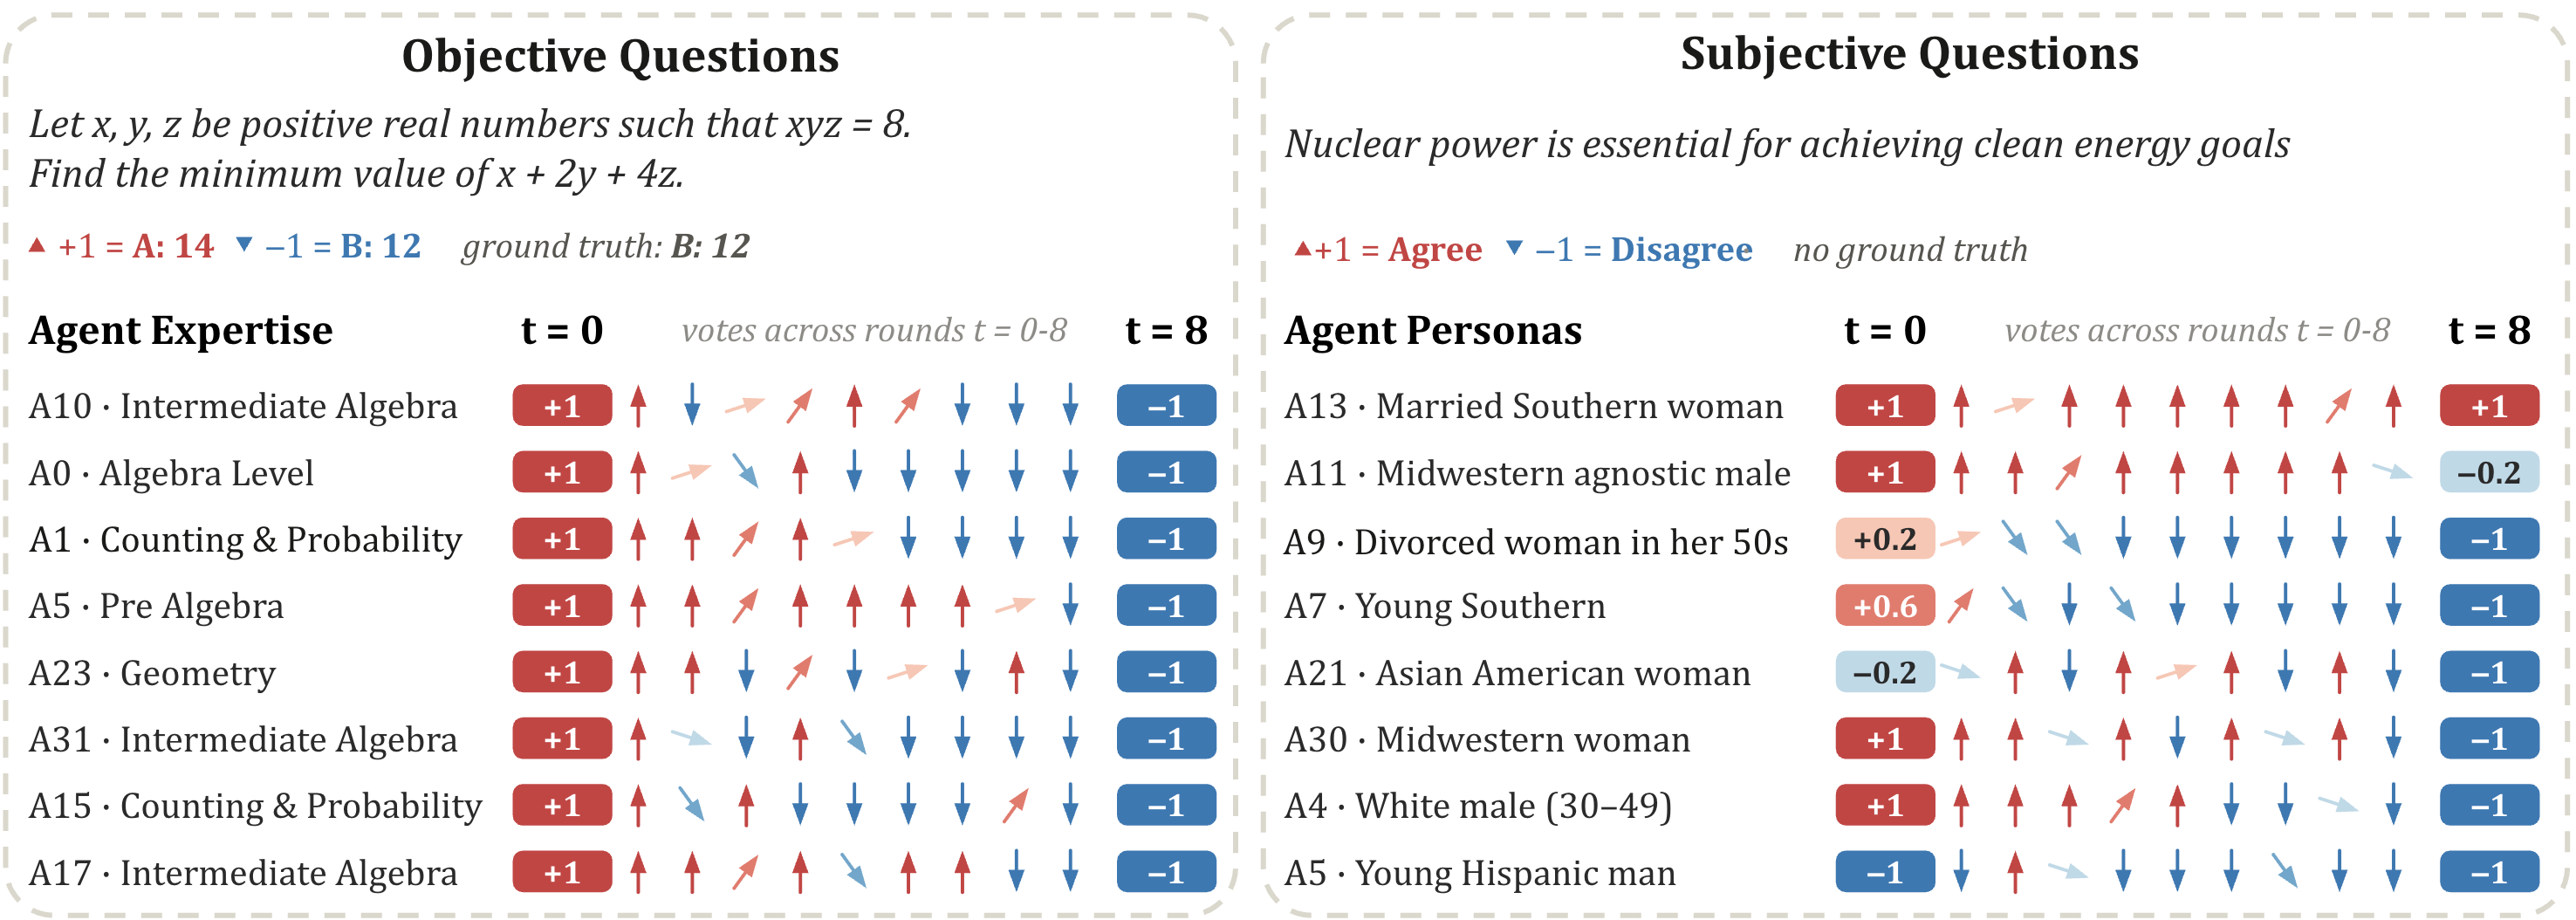
\includegraphics[width=0.99\textwidth]{main/Figures/apx_01_example_community_opinions.png}
    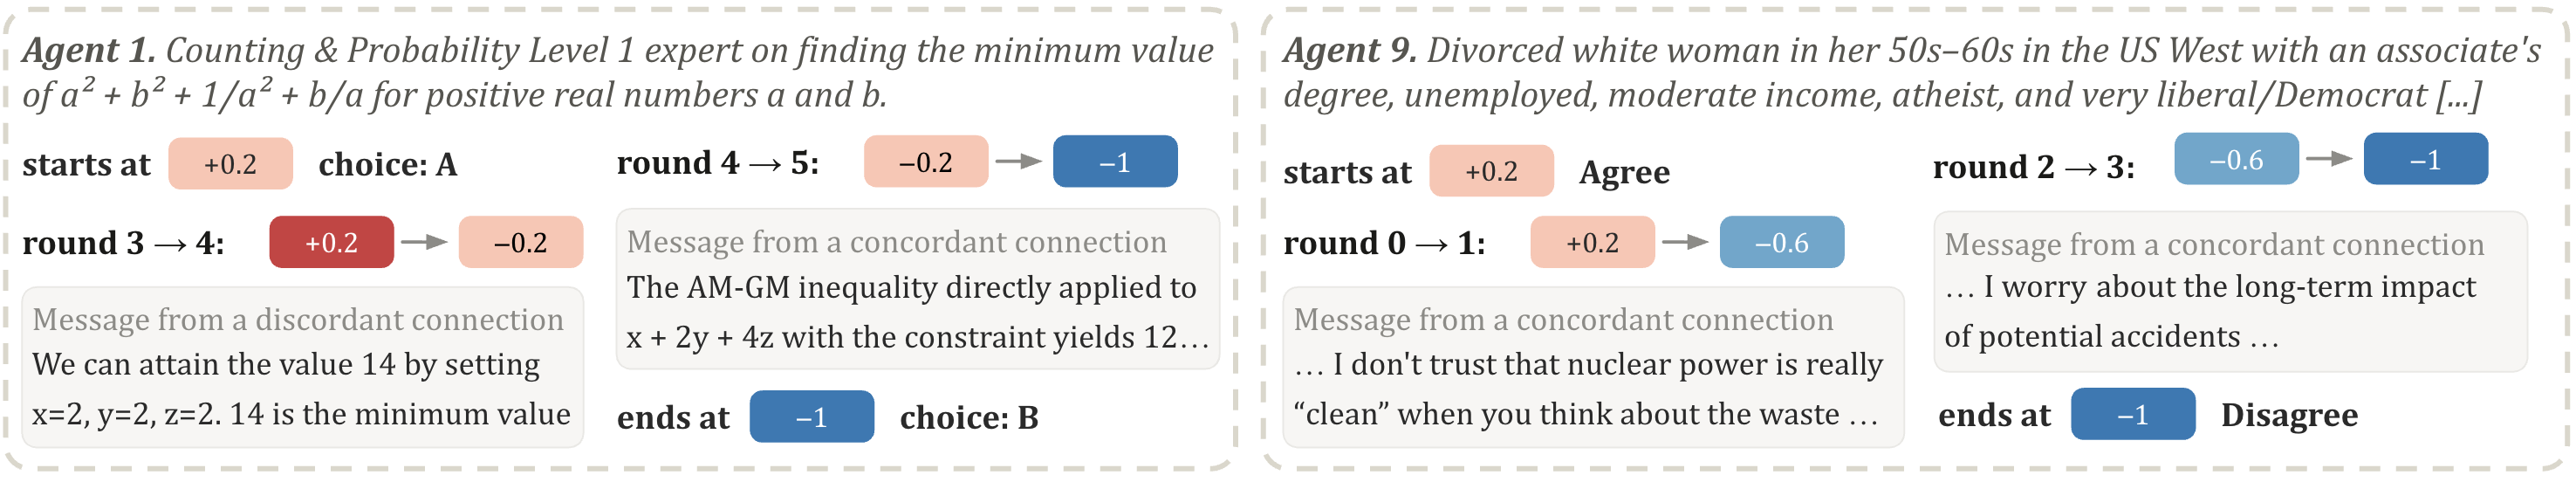
\includegraphics[width=0.99\textwidth]{main/Figures/apx_02_example_agent_messages.png}

   \caption{\textit{Example communities on an objective and a subjective questions.} \textit{Top:} opinions of eight agents over eight rounds of message exchange, from their initial vote at $t=0$ to their final vote at $t=8$; agents start out mostly agreeing on one side and end up on the other. \textit{Bottom:} two individual agents, showing the messages they received and the opinion changes that followed.}
\end{figure}

\textit{Subjective Questions.} Our subjective questions come from Political Questions Dataset for LLM Bias Evaluation \citep{promptfoo_political_bias_2025}\footnote{\url{https://huggingface.co/datasets/promptfoo/political-questions}}. We adapt the dataset to our experimental setting by reformulating each item as a political statement and asking the agent whether it agrees or disagrees with that statement, as illustrated in Figure~\ref{fig:prompt_overview}. The agent's response is restricted to one of two choices: \textit{agree} ($+1$), indicating agreement with the statement, or \textit{disagree} ($-1$), indicating disagreement with the statement. One example statement we examine is:
\begin{quote}\small
Mandatory vaccination violates bodily autonomy
\end{quote}


\textit{Subjective Personas.} We adapt \citet{toubia2025twin2k500datasetbuildingdigital} to our setup by extracting short free-text profiles using \texttt{gpt-4o-mini} from the dataset. These personas describe an individual along demographic and attitudinal axes,
including age, gender, ethnicity, region, marital and household status, education,
income, religiosity, political alignment, and personality and behavioral traits. For example:
\begin{quote}\small
You express the views of: Hispanic male in his 30s--40s living in the US West, single, agnostic, very liberal
Democrat, \dots\ highly empathetic and environmentally minded \dots
\end{quote}

\textit{Objective Questions.} Our objective questions come from the MATH dataset of
competition mathematics problems \citep{hendrycks2021measuringmathematicalproblemsolving}\footnote{\url{https://huggingface.co/datasets/hendrycks/competition_math}}. We adapt each problem to our experimental
setting by reformulating it as a binary multiple-choice question. The correct answer is
assigned to position \texttt{A} or \texttt{B} at random to remove positional bias. Each agent is shown the
problem together with two options, one of which is the correct final answer and the other a distractor. The agent is asked
which is correct, as illustrated in Figure~\ref{fig:prompt_overview}. The example below illustrates an objective question.
\begin{quote}\small
Find the distance between the foci of the hyperbola $x^2 - 6x - 4y^2 - 8y = 27.$\\
A: $4\sqrt{5}$ $\quad$ B: $4\sqrt{10}$
\end{quote}

\textit{Objective Personas.} Asking a language model to emulate a human persona while answering a mathematical question is of limited value, since the goal is to generate a mathematically correct answer. For this reason, we use questions from the MATH dataset \citep{hendrycks2021measuringmathematicalproblemsolving}, along with their ground-truth solutions, to construct objective expert personas. We note that it is more accurate to use the term \emph{expertise} when referring to objective personas.  Each agent is given the ground-truth solution to a unique question and therefore knows exactly how to solve that question correctly. The agent can then use this knowledge to help tackle a new problem. Each agent differs in their expertise. Below, we present an example objective persona.
\begin{quote}\small
You are a mathematics expert \dots here is one representative problem you have already solved correctly, together with its ground-truth solution \dots

Find the 6-digit repetend in the decimal representation of $\frac{3}{13}.$

Ground-truth solution:
We use long division to find that the decimal representation of $\frac{3}{13}$ is $0.\overline{230769},$ which has a repeating block of 6 digits. So the repetend is $\boxed{230769}.$
\end{quote}

\textit{Dataset Construction.} We construct both datasets through the two-step pipeline. \textit{(1) Binarization.} Every question is reduced to a binary choice. For the MATH problems, we prompt claude-4.8-opus \citep{anthropic2026opus48} to generate a plausible distractor for each question and assign the ground-truth answer and the distractor to choices A and B at random. For the political statements, the two choices are always Agree (+1) and Disagree (-1).  \textit{(2) High-entropy
filtering.} We then sample each of the $N=32$ agents eight times on every candidate question and keep the questions whose responses show the highest entropy across the repeated samples. We note that this step is necessary for observing interesting dynamics because  when a model produces the same answer on every sample, opinions are pinned from the outset and interaction has nothing to act on. In contrast, high-entropy questions exhibit non-trivial collective dynamics.

\textit{Train--test split.} The questions are split at random into equal halves. $20$ train and $20$ test objective questions, and $10$ train and $10$ test subjective
questions. For the objective set the split preserves label balance, with each
half containing $10$ questions whose correct answer is A and $10$ whose correct
answer is B. All fits use only train-question transitions, and all reported accuracies are on the test questions.

\subsection{Communication Networks}\label{apdx:communication_networks}
\begin{figure}[t]
    \centering
    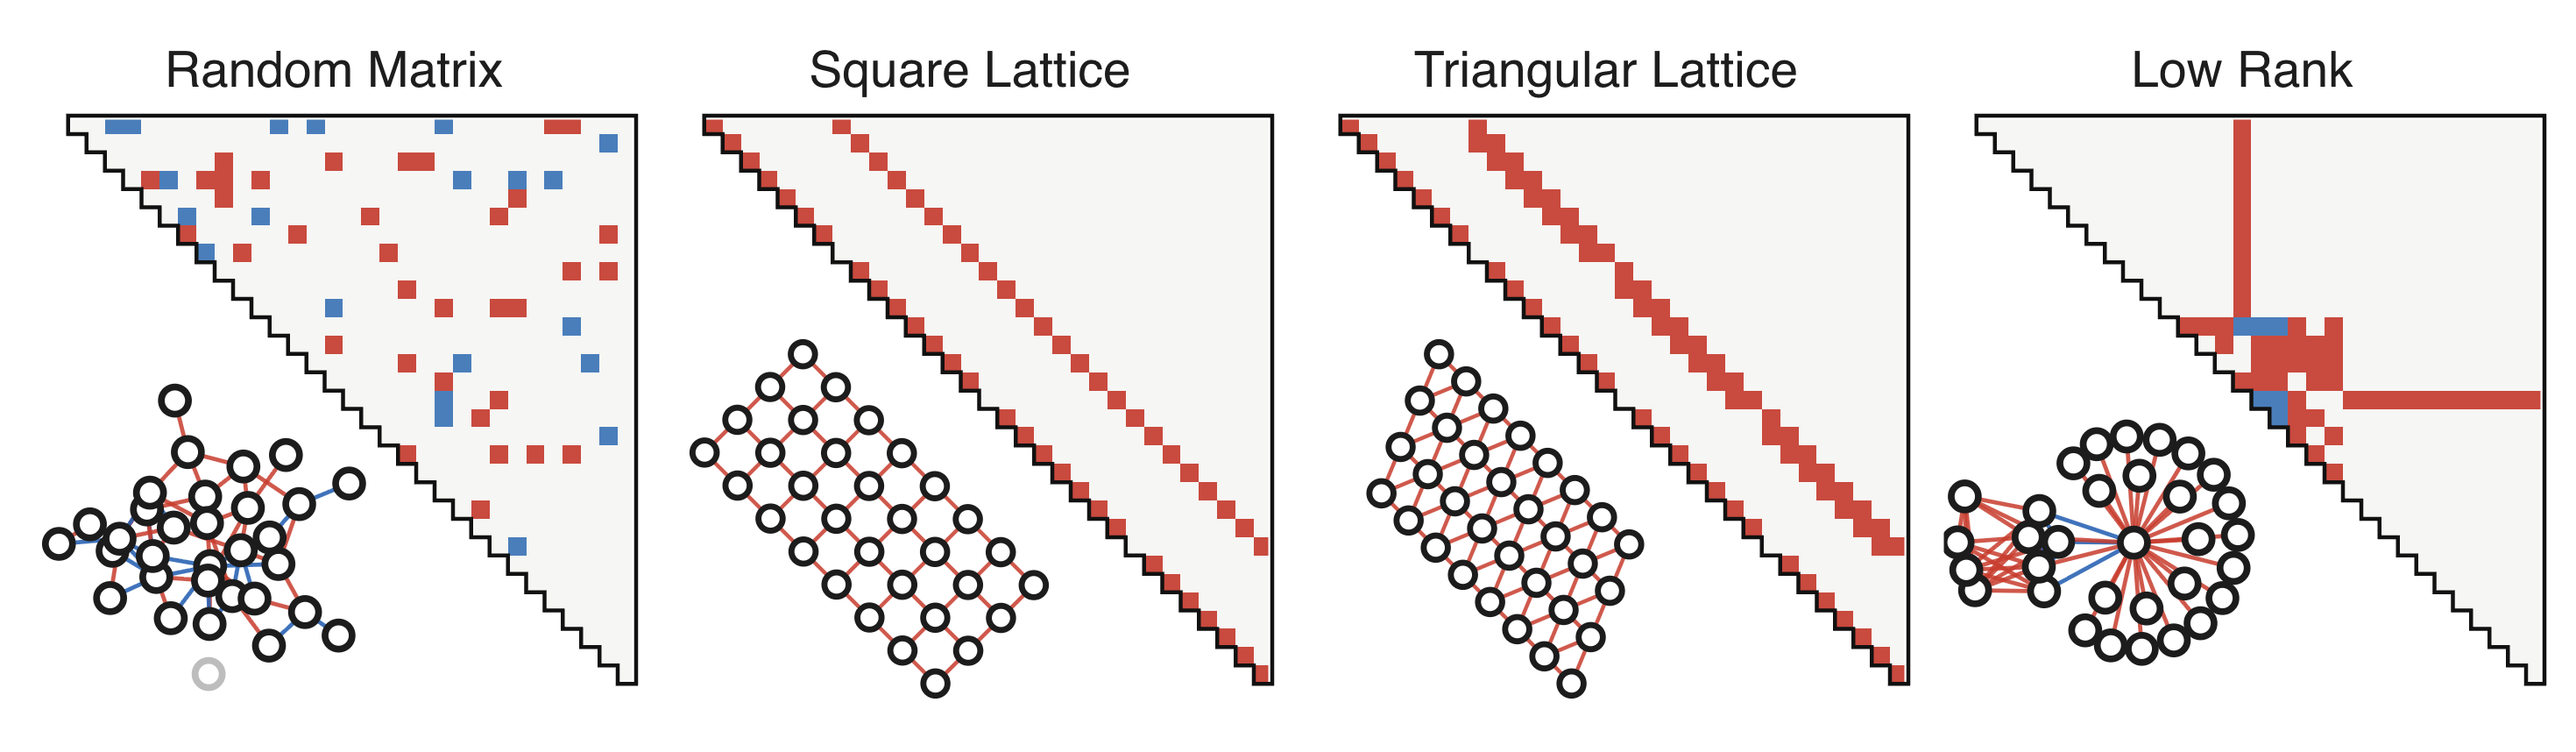
\includegraphics[width=0.99\textwidth]{main/Figures/apx_03_coupling_matrices.png}
    \caption{\textbf{Communication Networks: interaction matrix and graph structure.} Four structural families of communication networks (random matrices, square and triangular lattices, and low rank matrices) shown as the signed adjacency $J$ as a heatmap in one corner triangle (blue $-1$, white $0$, red $+1$) and as a node-link diagram. \label{fig:2_Setup_Js}}
\end{figure}

For our experiments, we generate the graphs $J$ from four families. \textit{(1) Random graphs (column 1 in Figure \ref{fig:2_Setup_Js})} are sampled with a fixed edge budget: for each unordered pair $i<j$ we draw $u_{ij}$ uniformly from (-1,1), and keep the pairs with the largest $|u_{ij}|$ until the edge budget is met, set $J_{ij}=\operatorname{sign}(u_{ij})$, and mirror to the lower triangle so that $J=J^{\top}$ with zero diagonal. We generate $12$ random graphs. \textit{(2) Lattices (columns 2 and 3 in Figure \ref{fig:2_Setup_Js})} are two deterministic, all-positive signed graphs reused across train and test: a square lattice (4-neighbor connectivity) and a triangular lattice (6-neighbor connectivity). \textit{(3) Rank- and frustration-controlled graphs (column 4 in Figure \ref{fig:2_Setup_Js})} aim to probe how the spectral structure of $J$ shapes the dynamics by varying two properties independently while holding the edge budget fixed. To test generalization of our model to low rank graphs, we generate a graph with a target \emph{algebraic rank} $\rho = 10$ and frustration densities $\gamma\in\{0.0,0.1,0.2\}$. We first build an all-positive signed graph whose adjacency has the prescribed rank, then introduce frustration by flipping the
signs of a fraction of edges until the frustration
density (the smallest fraction of edges left unsatisfied by any $\pm1$ opinion assignment) reaches $\gamma$. We draw two independent graphs per $(\rho,\gamma)$ cell, giving $1\times 3\times 2 = 6$ low rank graphs.

\subsection{Models}\label{apdx:models}

The backbone of the agents is a language model. We experiment with four different models: \texttt{gpt-4o-mini} \citep{openai2024gpt4ocard},
\texttt{gemma-3n-e4b-it} \citep{gemmateam2025gemma3technicalreport}, \texttt{qwen3.5-9b} \citep{qwen3.5},
and \texttt{llama-3.1-8b-instruct} \citep{grattafiori2024llama3herdmodels}. We run independent experiments with each model. Persona and question embeddings are computed
with OpenAI's \texttt{text-embedding-3-small} \citep{neelakantan2022textcodeembeddingscontrastive}.
